% !TEX encoding = UTF-8 Unicode

\documentclass{article}

\usepackage{imta_core}
\usepackage{imta_extra}
\usepackage[utf8]{inputenc}
\usepackage{caption}
\usepackage{subcaption}
\usepackage{amsmath,mathtools}
\usepackage[francais]{babel}
% \usepackage{bibtex}

\author{Wei GE \\ Yi QIAO}

\date{Mars 2018}
\title{Optimisation d’un portefeuille d’actifs par les réseaux de neurones}
\subtitle{Encadrant : \\   \\ Jean-Marc LE CAILLEC \\ Didier GUERIOT}

\imtaSetIMTStyle


%%%%%%%%%%%%%%%%%%%%%%%%%%%%%%% 
%%%%%%%%%% BEGINNING %%%%%%%%%% 
\begin{document}

\imtaMaketitlepage

\tableofcontents

\newpage


\section{Introduction}

Dans le marché financier, tout le monde cherche à gérer et optimiser son portefeuille pour obtenir le rendement attendu. Il y a une trentaine d'années, beaucoup de monde a commencé à essayer de prédire le rendement de l'action en utilisant le volume et les prix historiques, le prix le plus haut, le plus bas, d'ouverture et de clôture. Plus tard, des indicateurs techniques (TIs), qui représentent la tendance, la volatilité et l'ampleur du marché, ont été développés et calculés à partir de volume et de prix pour rendre la prédiction plus efficace.\\

Dans le cadre de notre projet, nous travaillons sur les données historiques de TI des actions dans l'indice CAC40 pour prédire le rendement en appliquant un modèle de réseaux de neurones. Il y a trois facteurs principaux qui vont impacter la prédiction du rendement, l'horizon, la longueur des données hisroriques utilisée et le nombre de TIs.\\

Dans la vraie vie, les investisseurs souvent font des opérations (par exemple, achat ou vent d'une action) pour manipuler leur portefeuille et laissent passer le temps sans prendre aucune mesure. Alors que cela peut être un bon choix lors de l'achat, et peut devenir de moins en monis performant au fils du temps. Par conséquent, il est très important de décider l'horizon approprié entre les deux opérations consécutives en prenant en compte le risque de la volatilité du marché, sachant qu'il est coûteux de faire des opérations fréquemment.\\

Comme nous travaillons sur des séries temporelles, qui d'ailleurs ne sont pas stationnaires de longue mémoire, il est intéressant de pouvoir déterminer la durée de données d'apprentissage pour mieux prédire le rendement à un horizon prédéfini, ainsi que le nombre de TIs.\\

Ce rapport est pour vous présenter notre projet en détail, qui contient 5 parties en global. D’abord, nous expliquons le context du projet, nous montrons notre problématique et les données fournies par nos encadrants. Ensuite, nous présentons le modèle de réseaux neurones pour réaliser la prédiction, qui consiste en la construction de la base d’apprentissage et les paramètres du modèle. Nous analysons les résultats obtenus et aussi évaluons notre modèle par les indicateurs statistiques. Dans la partie suivante, nous donnons des points à améliorer pour la continuation de ce projet. Ce rapport se termine par une conclusion synthétique. 


\subsection{Problématique}

Un portefeuille d'actifs est construit par plein d'actions des poids différents, les actions sont impactées par plusieurs facteurs comme le secteur, le pays, etc. Pour gérer un portefeuille d'actifs, l'objectif est de maximiser le rendement global, c'est-à-dire qu'il faut être capable de faire la décision d'acheter ou de vendre des actions pour optimiser le rendement de chaque action. Dans le cadre de notre projet, nous avons besoin d’optimiser d'un portefeuille CAC40. Comme les séries temporelles sont non stationnaires, donc il est très difficile de faire la prédiction pour chaque période.

\subsection{Présentation de données}

Le portefeuille CAC40 est construit par 49 actions françaises et chaque action a ses comportements complètement différents. Nous avons un fichier qui contient le prix (ouverture, clôture, haut, bas) et le volume de chaque action pendant presque 15 ans (2000-2015). Les données dans ce fichier seront utilisées pour calculer le rendement d'un horizon déterminé. Pour une série temporelle, si nous prenons une période trop courte, nous n'aurons pas assez d'informations pour faire la prédiction. En revanche, elle n'a pas une forte corrélation pendant une longue période, les données très anciennes ne sont pas utile de prédire la situation actuelle.\\

Nous avons aussi un fichier ayant les 13 « technical indicators » calculés à partir de ces séries temporelles. Les TIs se situent dans 4 catégories : le volume, la volatilité, la tendance et le momentum.


\newpage



\section{Conception et développement du modèle}

La prédiction du prix d'une action ou son rendement par une série temporelle financière fait l'objet de nombreuse recherches. Les investisseurs ont pris beaucoup de modèles différents pour la prédiction du prix d'action basée sur les informations historiques. Ils voudraient bien savoir la hausse et la baisse du marché financier pendant une période. Maintenant, il y a plusieurs techniques pour réaliser cette tâche, comme support vector machines (SVMs), case-based reasoning (CBR) et artificial neural networks (ANNs). \footnote{Kyoung-jae Kim, Financial time series forecasting using support vector machines, Department of Information Systems, College of Business Administration, Dongguk University, 2003} \\

Pour atteindre notre objectif, nous avons proposé le modèle de réseaux de neurones pour faire la prédiction. L’entrée et la sortie de notre projet sont très différentes par rapport aux autres projets. Les entrées sont les 13 TIs, comme nous le savons, avoir plus de TIs permet d'obtenir plus d’informations, mais il y a aussi plus de risques d’avoir trop de redondances en prenant plusieurs TIs de la même catégorie. La sortie est le rendement à un horizon prédefini, il est plus difficile de prédire la vraie valeur que la tendance (mettre une seuil comme signal d’achat ou de vente). Dans cette partie, nous présentons la façon de construction de la base d'apprentissage, le pré-traitement sur les données d'origines et les paramètres de la base d'apprentissage. 

\subsection{Construction de la base d’apprentissage}

La base d'apprentissage en entrée du réseau de neurones est composée de patterns, et chaque pattern représente les données d'un jour, qui contient 13 TIs : 5 TIs qui indiquent la tendance du marché, 3 TIs qui représentent l'ampleur, 3 TIs qui expriment la volatilité et 2 TIs qui symbolisent le volume. Comme notre modèle d'apprentissage de la prédiction du rendement est supervisé, nous avons besoin d’ajouter les labels pour les patterns correspondants, c’est-à-dire qu'il faut calculer le rendement à un certain horizon pour chaque pattern. La formule permettant de calculer le rendement est $ r = \frac{P_{t_{0}+h_{0}}}{P_{t_{0}}} - 1 $.


\subsubsection{Pré-traitement de données}

Les données de 13 TIs sont sur des échelles différentes. Dans un premier temps, nous avons utilisé directement ces données calculées, parce que nous avions supposé que notre modèle de réseaux de neurones est capable de s'adapter pour les normaliser, cela signifie que les grandes valeurs ne vont pas être considérées comme plus importantes que les petites. Cependant, quand nous avons fait le premier test sur ces données, nous avons eu un résultat qui n’était pas idéal. Le réseau de neurones n'a pas réussi à apprendre l'évolution de la courbe de rendement et la prédcition est loin d'être bonne. Ensuite, nous avons normalisé ces entrées en utilisant la formule $ V_{normalize} = \frac{V-V_{min}}{V_{max}-V_{min}}$, ainsi les valeurs de 13 TIs ont été ramenées dans une fourchette de [0,1]. Dans ce cas, le poids attribué à chaque TI dont le réseau tient compte est correct. Après avoir appliqué la normalisation, le résultat est meilleur et la valeur de prédiction s'est approchée vers la vraie valeur. \\

La figure \ref{fig: normalisation} vous montre la différence entre les données normalisées et non mormalisées, nous avons appliqué cette démarche à la base d'apprentissage et la base de test. Nous pouvons constater que notre système peut bien apprendre les données normalisées dans la base d'apprentissage. Dans la base de test, même si le résultat de prédiction n'est pas parfait, les données normalisées suivent la vraie valeur. En revanche, les données non normalisées n'ont jamais appris la tendance sur le vrai rendement. 

\begin{figure}[H]
\centering
	\begin{subfigure}{.5\textwidth}
	\centering
	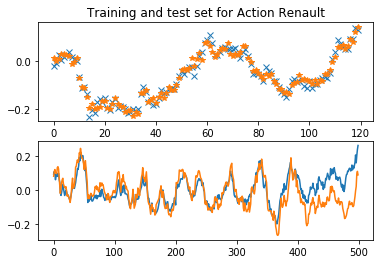
\includegraphics[width=.9\linewidth, scale=0.2]
	{plot/norma.png}
	\caption{Données dans la base d'apprentissage}
	\label{fig:Base_A}
	\end{subfigure}%
	\begin{subfigure}{.5\textwidth}
	\centering
	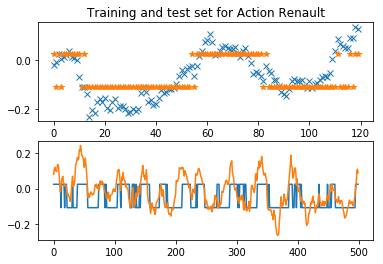
\includegraphics[width=.9\linewidth, scale=0.2]
	{plot/non_norma.png}
	\caption{Données dans la base de test}
	\label{fig:Base_T}
	\end{subfigure}
\caption{Comparaison entre les données non normalisés et normalisés sur les 2 bases}
\label{fig: normalisation}
\end{figure}

\subsubsection{Paramétrage de la base d'apprentissage}

Pour notre projet, il faut aussi faire varier les différents paramètres pour construire la base d'apprentissage, qui sert à tester des différents scénarios. Nous prenons principalement 4 paramètres pour comparer le résultat de chaque scénario : l'horizon, la taille d'apprentissage, la durée du test et le nombre de TIs. Pour lancer des tests sur les différents scénarios, nous faisons chaque fois varier seulement un paramètre afin de trouver la meilleure combinaison de paramètres.\\

Comme nous avons besoin de prédire le rendement dans un horizon, il faut prendre horizon plus de prix pour calculer les derniers rendements dans la base d'apprentissage. Nous avons commencé le test après un décalage de horizon, c'est-à-dire que nous ne pouvons pas utiliser les données just après pour faire le test. Dans notre projet, nous pouvons considérer la période de décalage comme la base de validation. La figure \ref{fig:BA} est une illustration plus claire : \\

\begin{figure}[H]
	\centering
	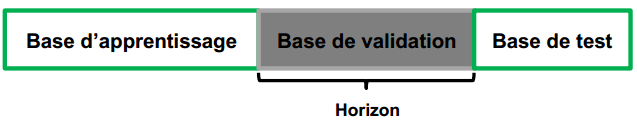
\includegraphics[width=.5\linewidth, scale=0.2]
	{plot/BA.png}
	\caption{Construction de la base}
	\label{fig:BA}
\end{figure}

Nous avons pris tous les 13 TIs au début de notre projet, nous voudrons collecter plus d’informations pour faire la prédiction, nous avons considéré que cette combinaison de TIs est plus robuste. Pour savoir si le nombre de TIs a un impact sur la performance de notre système, nous avons diminué le nombre de TIs et refait des tests avec la dimension réduite en entrée du réseau. Les nombres de TIs que nous avons choisi sont 13, 12 (élimination d'un TI) et 4 (un TI par catégorie).

\subsection{Choix du modèle}

De nombreuses études ont largement admis que la non-linéarité existe sur les marchés financiers et que les réseaux de neurones peuvent être efficacement utilisés pour découvrir cette relation. Les modèles de réseaux de neurones pour l'estimation sont ensuite examinés pour leur capacité à fournir une prévision efficace des valeurs futures.\\

Nous avons utilisé l'algorithme de perceptron multicouche à rétropropagation. Le perceptron multicouche est un type de réseau organisé par plusieurs couches, chaque couche est constituée d'un nombre variable de neurones, les neurones de la dernière couche étant les sorties du système global. Dans notre cas, l'entré de reseau est les TIs et la sortie est le rendement de l'action. L'algorithme de rétropropagation du gradient déscendant est pour minimiser l'erreur afin de converger. Les figures \ref{fig:RN} et \ref{fig:base} représentent la structure de notre réseau de neurones et nos examples d'entrées en format matriciel :\\

\begin{figure}[H]
	\centering
	\begin{subfigure}{.5\textwidth}
	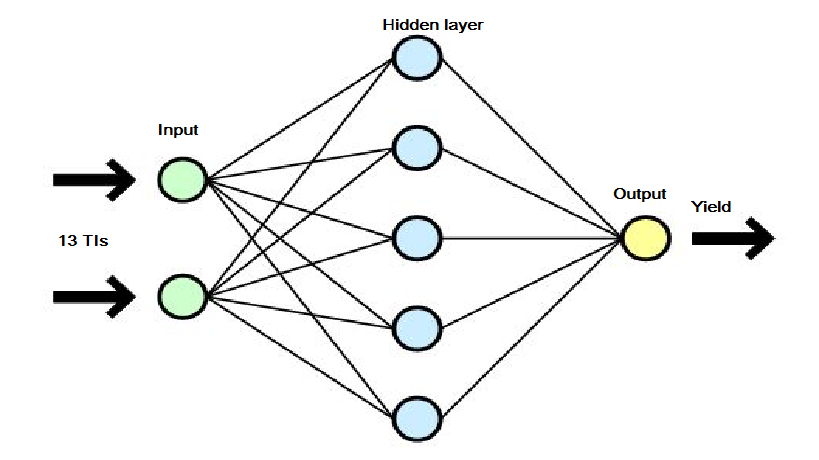
\includegraphics[width=.9\linewidth, scale=0.2]
	{plot/RN.png}
	\caption{Structure de réseaux neurones}
	\label{fig:RN}
	\end{subfigure}%
	\begin{subfigure}{.5\textwidth}
	\centering
	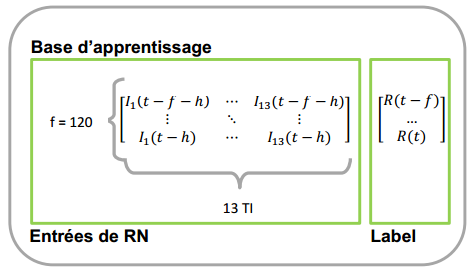
\includegraphics[width=.9\linewidth, scale=0.2]
	{plot/base.png}
	\caption{Entrée de base d'apprentissage}
	\label{fig:base}
	\end{subfigure}
\caption{Structure du modèle de perceptron multicouche à rétropropagation}
\label{fig:structure_rn}
\end{figure}

Dans le modèle de réseaus neurones, nous avons besoin de choisir le nombre de neurones, le nombre de couches cachés, le taux d'apprentissage, la fonction d’activation et le nombre d'itération. Pour notre projet, nous avons pris une seule couche cachée avec 25 neurones et nous avons paramétré le taux d'apprentissage initial égale à 0,1. Nous avons pris la fonction sigmoid $ f(x) = \frac{1}{1 + exp^{-x}} $ comme la fonction d'activation, ainsi notre nombre d'itération est 80000.

\subsection{Préparation des scénarios}

Pour lancer les simulations différentes, nous n'avons changé qu'un seul indicateur dans chaque scénario de test. Comme nous avons dit avant, il y a 4 paramètres pour construire notre base d'apprentissage. Nous avons préparé les scénarios en variant sur un des indicateurs pour choisir une valeur plus favorable pour chaque paramètre. \\

En général, la contrainte de la prédiction d'une série temporelle est la non stationnalité de données, nous ne pouvons pas utiliser les données non corrélées pour faire la prédiction, donc il faut bien défini la durée d'apprentissage. Par conséquent, nous avons besoin de savoir le nombre de patternes à apprendre, si nous prenons trop de patternes, il y a un coût d'apprentissage très élevé et aussi il peut produire le problème de sur-apprentissage. Cependant, si nous prenons pas assez de patternes, la base ne peut pas générer la bonne prédiction, parce qu'elle n'a pas assez d'examples à s'entraîner. \\

Pour savoir la féquence de la gestion de portefeuille, il faut varier sur l'horizon de rendement. Le mouvement du marché est plus petit pendant un horizon plus court, mais dans la réalité nous ne pouvons pas relancer un portefeuille très fréquemment. Par contre, si nous utilisons un horizon plus long, il y a un risque d'avoir une performance très mauvaise. \\

La base de test est pour vérifier le résultat de l'apprentissage et aussi pour mesurer la performance de prédiction. Nous varions sur la taille de test pour savoir pendant combien de temps maximum le modèle est toujours valable et s'il y a un recyclage sur les valeurs prédites. \\

Dans un premier temps, nous prenons tous les 13 TIs pour les autres scénarios, mais il faut aussi considérer l'influence du nombre de TIs. Nous allons caluler la corrélation entre les 13 TIs et essayer de réduire la dimension de nombre de TIs. Dans l'article \footnote{J. M. Le Caillec, A. Itani, and D. Guriot, Stock Picking by Probability–Possibility Approaches, IEEE TRANSACTIONS ON FUZZY SYSTEMS, VOL. 25, NO. 2, APRIL 2017}, elle propose plusieurs de combinaisons pour les TIs. Les combinaisons plus intéréssantes sont tous les 13 TIs, les 12 TIs (sauf EMA), les 4 TIs (un par catégorie, soit SMA,CCI,BB1,EMV).\\

Dans la partie suivante, nous vous présentons nos résultats par les différents types de scénarios. En parallèle, nous montrons les explications plus raisonables pour mettre un vrai sens à notre projet. Ensuite, nous avons aussi besoin d'évaluer la performance de notre modèle de prédiction.




  






 
\newpage


\section{Résultats obtenus et analyse}
 
\subsection{Résultats de différents scénarios}

\subsubsection{Variation de taille d'apprentissage}
Comme nous travaillons sur des séries temporelles, qui ne sont pas stationnaires, nous nous intéressons à l'effet de la taille d'apprentissage sur la précision de la prédiction du rendement de l'action. Nous avons réalisé des tests sur l'action Renault dans l'indice CAC40.\\

Sur la figure \ref{fig:SE_Trainingset}, nous observons un très grand pic au début d'octobre 2008 avec une taille d'apprentissage de 120 jours (6 mois), juste après le début de la crise mi-septembre. Toutefois, ce pic est absent sur les autres courbes. Cela signifie que notre modèle est capable de détecter le début de la période de la crise, puisqu'une fois que celle-ci est arrivée, la tendance du marché est brutalement rompue. Dans ce cas, apprendre sur les données des 6 derniers mois n'est pas une bonne approche pour la prédiction du rendement. En revanche, apprendre sur une période plus courte est plus efficace pour ne prendre en compte que les informations intéressantes de l'évolution du marché.\\

Dans les autres périodes, nous pouvons constater que l'erreur quadratique de la prédiction du rendement est proche de zéro dans les quatre cas.

\begin{figure}[H]
\centering
\begin{subfigure}{.5\textwidth}
\centering
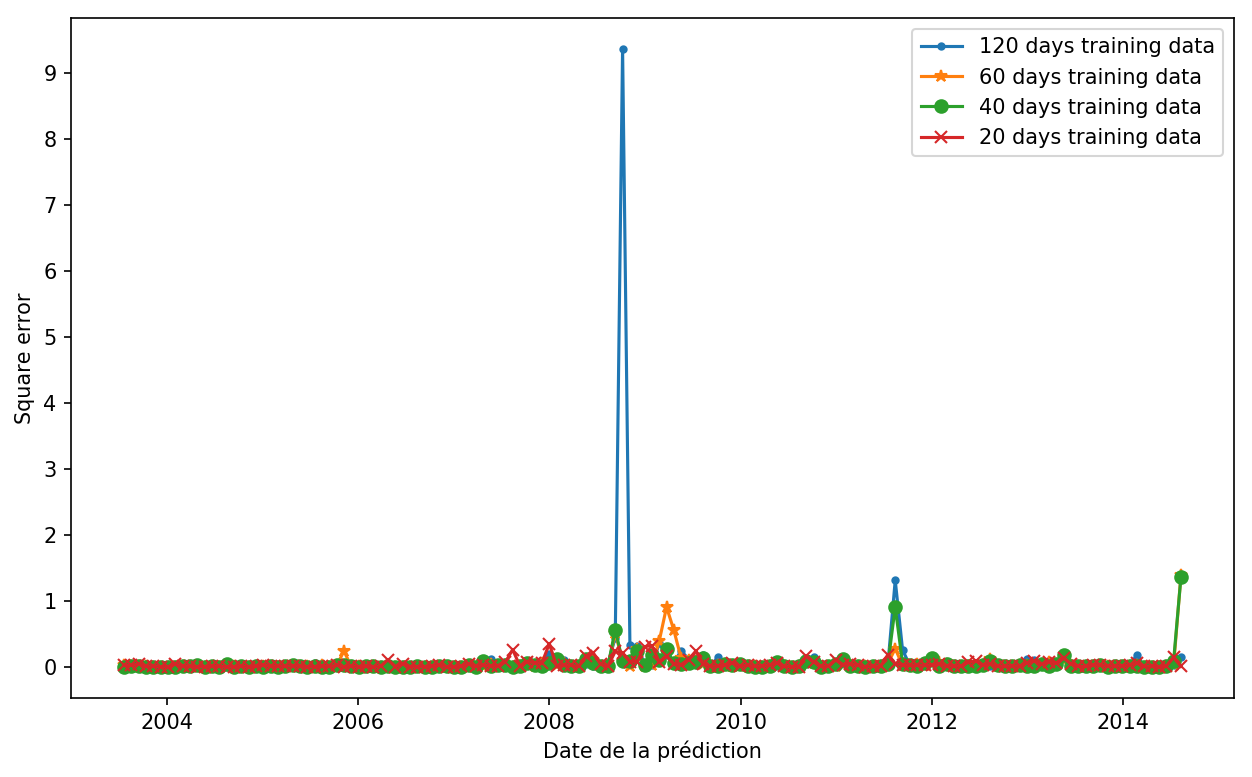
\includegraphics[width=.9\linewidth, scale=0.2]
{plot/SE_Trainingset.png}
\caption{Vue globale sur 10 ans}
\label{fig:SE_Ts1}
\end{subfigure}%
\begin{subfigure}{.5\textwidth}
\centering
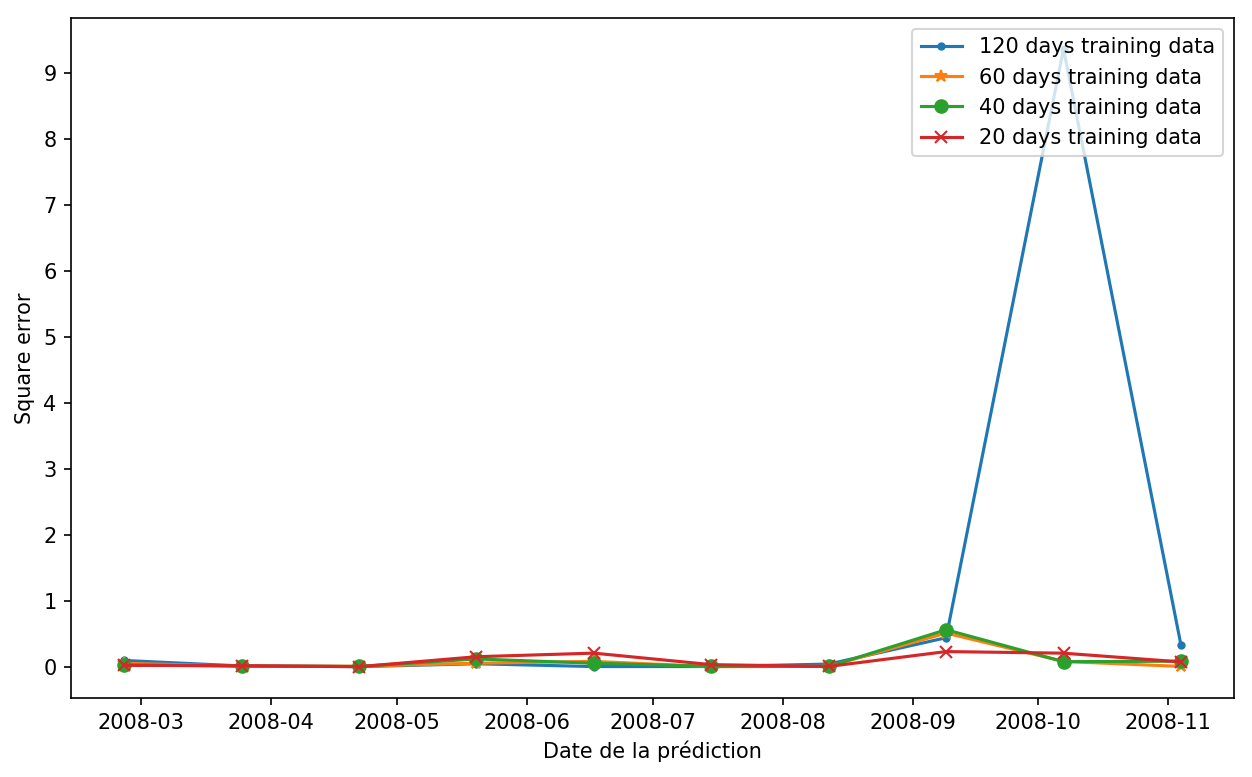
\includegraphics[width=.9\linewidth, scale=0.2]
{plot/SE_Trainingset_s.png}
\caption{Vue zoomée sur la période de la crise de 2008}
\label{fig:SE_Ts2}
\end{subfigure}
\caption{Erreur quadratique de la prédiction du rendement de Renault à un horizon de 20 jours (1 mois) en fonction de la taille d'apprentissage}
\label{fig:SE_Trainingset}
\end{figure}

En observant les figures ci-dessous, nous remarquons que l'erreur moyenne pour 120 jours est généralement plus petite que les autres cas (sauf la période de la crise), car une periode plus longue contient plus d'informations et peut mieux présenter la tendance du marché. Au contraire, une période plus courte est plus bruitée.

\begin{figure}[H]
\centering
\begin{subfigure}{.5\textwidth}
\centering
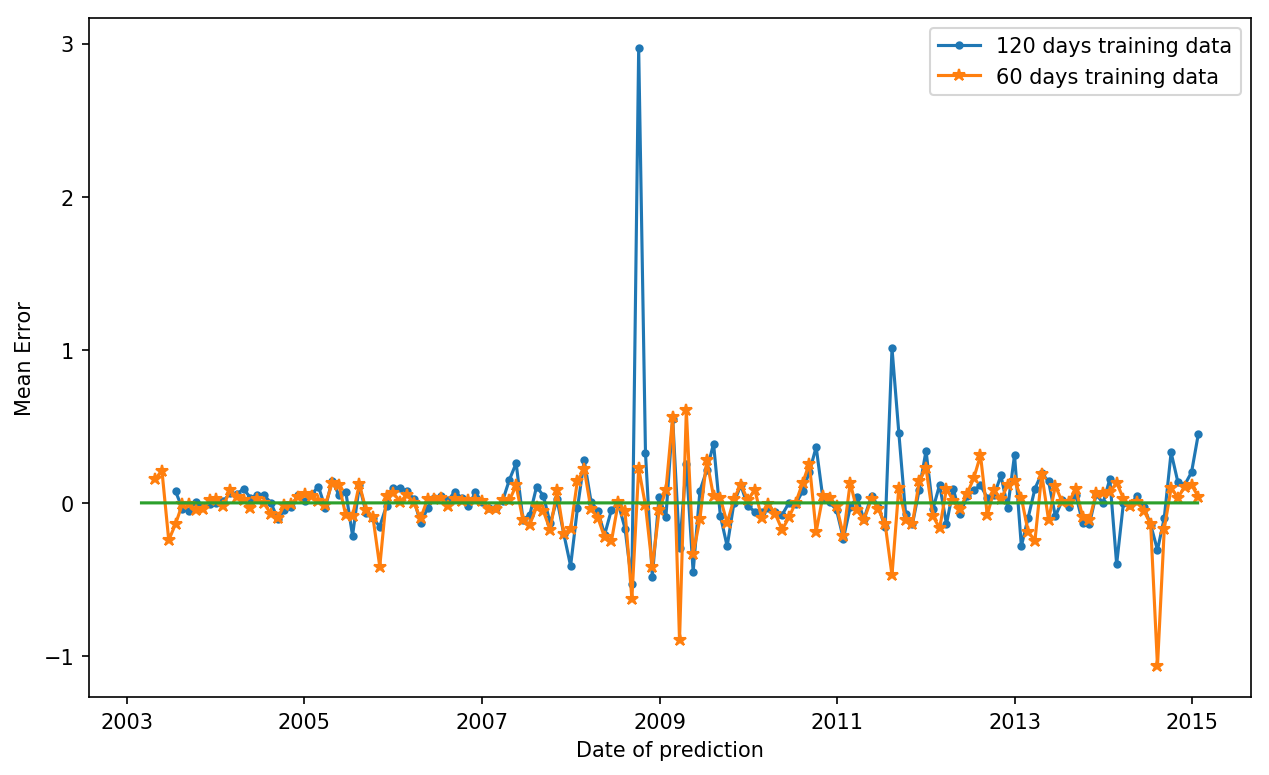
\includegraphics[width=.9\linewidth, scale=0.2]
{plot/ME_Trainingset1.png}
\caption{Erreur moyenne pour 120 et 60 jours}
\label{fig:ME_Ts1}
\end{subfigure}%
\begin{subfigure}{.5\textwidth}
\centering
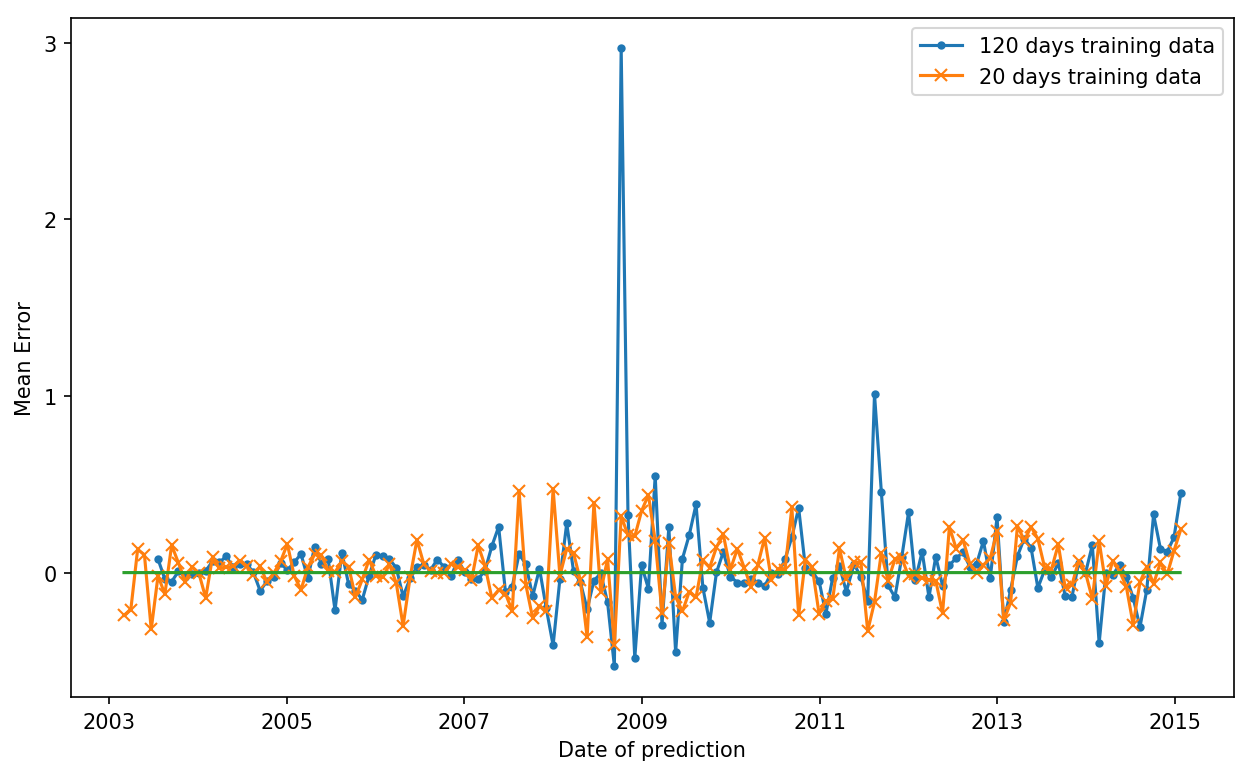
\includegraphics[width=.9\linewidth, scale=0.2]
{plot/ME_Trainingset2.png}
\caption{Erreur moyenne pour 120 et 20 jours}
\label{fig:ME_Ts2}
\end{subfigure}
\caption{Erreur Moyenne de la prédiction du rendement de Renault à un horizon de 20 jours (1 mois) en fonction de la taille d'apprentissage}
\label{fig:ME_Trainingset}
\end{figure}


\subsubsection{Variation de l'horizon}




\subsection{Evaluation du modèle}

\subsection{Difficultés rencontrées}


L’apprentissage a pris trop de temps.

Trop de scénarios

Bcp d’actions

 

\newpage
 
\section{Difficultés rencontrées et points à améliorer}

\subsection{Difficultés rencontrées}
Les marchés financiers ne sont pas du tout stables, ni prévisibles, et même un message de Twitter peut les influencer. Par conséquent, il est difficile de prévoir le rendement d'une action sur le marché. De plus, la performance d'une action varie beaucoup, non seulement en fonction de facteurs économiques tels que le taux d'intérêt et l'inflation, mais aussi en fonction du secteur où elle se trouve, la taille de l'entreprise, les activités des entreprises concurrentes, et cætera.\\

Nous travaillons sur les actions européennes dans l'indice CAC40 qui est composé de 49 actions de différents secteurs : banque et assurance, transports, technologie, études et conseil, et cætera. Appliquer notre modèle de prédiction à toutes ces actions et comparer les résultats des autres actions du même secteur représente donc un projet conséquent. De plus, l'outil que nous utilisons pour l'implémentation est iPython notebook. Son avantage est qu'il est aisé d'y réaliser des tests et de visualiser les résultats, mais il n'est pas très efficace pour lancer de nombreux tests de différents scénarios et pour vérifier la performance du modèle.\\

\subsection{Points à améliorer}
Nous avons réussi à réaliser tous les tests sur l'action de Renault, de PSA et d'Alcatel-Lucent. Les travaux futurs seront d'améliorer la performace de notre modèle pour minimiser l'erreur de la prédiction, par exemple, d'implémenter les autres scénarios potentiels pour trouver une meilleure combinaison de paramètres pour le modèle. Il est aussi intéressant d'appliquer notre modèle de prédiction à toutes les autres actions pour voir si sa capacité de prédiction est générique.\\

L'objectif final de notre modèle est de permettre aux traders de prendre des décisions à un horizon donné, d'acheter, de vendre ou de ne rien faire sur les actions dans leur portefeuille afin d'optimiser ce dernier. C'est un travail à réaliser à partir du modèle actuel. Par ailleurs, nous proposons d'implémenter l'algorithme en C++ pour qu'il soit plus déterministe et efficace une fois le modèle amélioré.
 
\newpage
 

\section{Conclusion}

Ce projet constitue une belle opportunité pour découvrir la nouvelle technique pour prédire la séries temporelle, cela nous permettra d’acquérir des connaissances sur le réseau de neurones et les événements financiers. Il s’est déroulé du 23 octobre 2017 au 14 mars 2018, nous avons commencé par la compréhsion du sujet et les recherches. Ensuite, c'est une phase de conception, nous avons discuté beaucoup sur les paramètres de la base, puisque cela est lié significativement à la performance du modèle. Le plus important est la phase de test, nous avons commencé à faire des analyses et les relier avec les événements dans la vraie vie. Cependant, nous avons eu beaucoup de difficultés dans cette période, parce que le temps d'exécution est trop long, ainsi les résultats sont très variés. Nous n'avons pas réussit à faire tous les tests sur toutes les actions, par contre nous avons déjà obtenu un premier résultat global sur l'action Renault. Nous pensons que pour aller plus loin, il faut continuer à tester les scénarios sur tous le portefeuille de CAC40. \\

Au point de vue personnelle, nous avons pratiqué beaucoup l'analyse et la prédiction de données sous ipython, c'est utile pour la vie professionnelle dans le futur. Même s'il est très difficile d'avoir un résultat idéal, nous avons déjà appris plein de démarches pour déployer ce genre de sujet. Il vaut mieux avoir plus de temps pour finir tous les tests, ainsi que les comparaisons entre les différents cas. 

\end{document}
%%%%%%%%%% END %%%%%%%%%% 
%%%%%%%%%%%%%%%%%%%%%%%%% 
